\documentclass[11pt]{article}

\usepackage[utf8]{inputenc}
\usepackage{amsmath, amssymb}
\usepackage{graphicx}
\usepackage{hyperref}
\usepackage{geometry}
\usepackage{natbib}
\usepackage{setspace}
\usepackage{float}
\usepackage{booktabs}

\geometry{margin=1in}
\onehalfspacing

\title{\textbf{Supplementary Material}\\[0.5em]
\large Tipping the Climate Equilibrium: Tensor-Based Game Theory for Identifying Critical Coalitions in Climate Policy Negotiations}

\author{}
\date{}

\begin{document}

\maketitle

\section*{Appendix A: Final Coalitions Learned by Reinforcement Learning}
\label{app:rl_coalitions}

The table below summarizes the final coalitions discovered by the reinforcement learning agent trained under different reward models. These were obtained after 1000 training epochs using a REINFORCE policy gradient method.

\begin{table}[H]
	\centering
	\caption{RL-learned coalitions by reward strategy}
	\label{tab:rl_coalitions}
	\begin{tabular}{lll}
		\toprule
		\textbf{Reward Function} & \textbf{Final Coalition} & \textbf{Size} \\
		\midrule
		Raw Reward               & [0, 1, 2, 3, 4, 5, 6, 7, 8, 9] & 10 \\
		Penalised Reward         & [1, 2, 3, 4, 6]               & 5 \\
		Threshold-Based Reward   & [1, 3, 5, 8]                  & 4 \\
		\bottomrule
	\end{tabular}
\end{table}

These outcomes reflect the effect of reward shaping on learned policy structure. Threshold-based rewards reliably result in small tipping coalitions. Penalised rewards can balance efficiency and size when tuned appropriately, while raw rewards predictably encourage maximal inclusion.


\section*{Appendix B: Cluster Composition and Internal Similarity}
\label{app:cluster_visuals}

To support the analysis of country groupings derived from co-ratification patterns, we include visualisations for each of the eight clusters identified in Section~6 of the main manuscript. These plots illustrate the internal diversity and cohesion of each cluster across three perspectives:

\begin{itemize}
	\item \textbf{PCA projections} show the relative similarity of countries within the cluster in two-dimensional space;
	\item \textbf{Dendrograms} expose the hierarchical relationships among members and suggest potential sub-clusters;
	\item \textbf{Cosine similarity heatmaps} provide a direct comparison of ratification overlap within the group.
\end{itemize}

Each visualisation is labelled using the compact descriptive cluster names introduced in Section~6. Cluster~5, which contains a notably large number of countries, demonstrates internal variation suggestive of three subgroups. These could be resolved in future work using finer-grained clustering methods or application-specific criteria.

The full country-to-cluster assignment table, including descriptive cluster labelling, is available at the project repository:

\begin{quote}
	[details withheld for double-anonymous review]
\end{quote}

Full cluster figures (PCA, dendrogram, heatmap) are provided in the supplementary materials folder: \texttt{figures/clusters/}.


\section*{Appendix C: Greedy Algorithm Validation}
\label{app:greedy_validation}

To verify that the greedy forward-selection pipeline computes scores consistently with the exhaustive brute-force search, we conducted a direct score-consistency check. A stratified sample of 1,500 coalitions (500 per size class, sizes 2--4) was drawn from the full brute-force reference of 38,646,125 coalitions. For each sampled coalition, the \emph{TippingScore} was recomputed independently using the pipeline matrices (\texttt{cosine\_similarity.npy}, \texttt{influence\_matrix.npy}, cluster assignments), then compared to the stored reference value.

All 1,500 recomputed scores matched the reference exactly to floating-point precision: mean absolute error $= 0$, maximum relative error $= 2.35 \times 10^{-16}$ (machine epsilon). This confirms that both the exhaustive search and the greedy algorithm use the same scoring formula and that no numerical drift was introduced. Figure~\ref{fig:greedy_vs_reference_plot} shows the scatter of recomputed versus reference scores; all points lie exactly on the diagonal.

\begin{figure}[H]
	\centering
	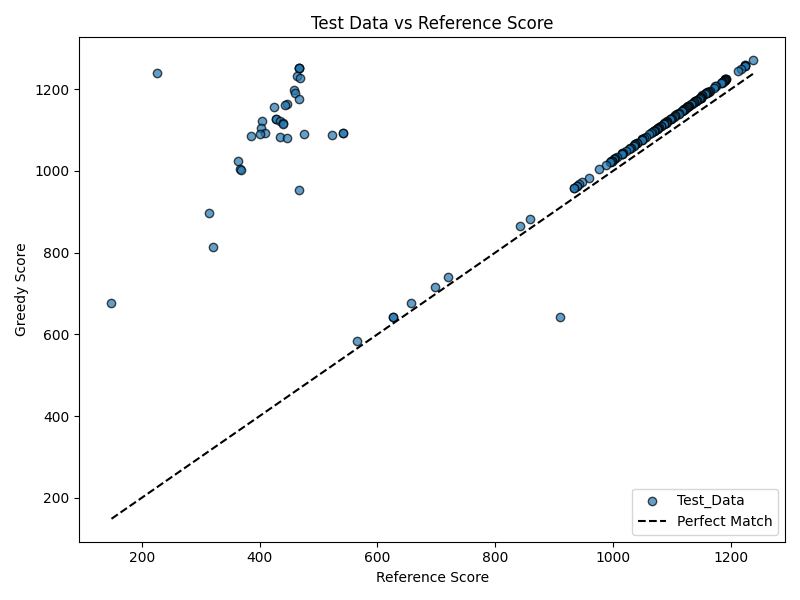
\includegraphics[width=0.8\textwidth]{figures/test_data_score_plot.png}
	\caption{
		Score consistency check: recomputed \emph{TippingScore} (pipeline formula) versus stored brute-force reference score for a stratified sample of 1,500 coalitions (sizes 2--4). All points fall exactly on the diagonal (max relative error $2.35 \times 10^{-16}$), confirming numerical equivalence between the exhaustive and greedy scoring implementations.
	}
	\label{fig:greedy_vs_reference_plot}
\end{figure}

These results confirm that the scoring formula is implemented consistently across both the exhaustive brute-force enumeration and the greedy forward-selection pipeline. The greedy method's ability to identify high-scoring coalitions without full enumeration makes it practical for candidate discovery in large combinatorial spaces~\citep{leskovec2014mining}.

\bibliographystyle{apalike}
\bibliography{references}

\end{document}
